% vim: set textwidth=78 autoindent:

% when the revision of a section has been finalized,
% comment out the following line:
%\updatedisclaimer

\section{Map Production}\label{sec:mapproduction}
\begin{tabular}{p{3.5cm}p{6cm}p{6cm}}
\multirow{2}{*}{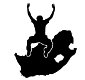
\includegraphics[width=2.5cm]{logo}} & Objectives: &
Understanding of map production for spatial data. \\
& & \\
& Keywords: & 
Map production, map layout, scale bar, north arrow, legend, map body, map
unit  \\
\hline
\end{tabular}

\subsection{Overview}

\textbf{Map production} is the process of arranging map elements on a sheet of paper
in a way that, even without many words, the average person can understand
what it is all about. Maps are usually produced for presentations and reports
where the audience or reader is a politician, citizen or a learner with no
professional background in GIS. Because of this, a map has to be effective in
communicating spatial information. Common elements of a map are the \textbf{title,
map body, legend, north arrow, scale bar, acknowledgement}, and \textbf{map
border} (see Figure \ref{fig:mapelements}).

\begin{figure}[ht]
   \begin{center}
   \caption{Common map elements (labelled in red) are the title, map body,
legend, north arrow, scale bar, acknowledgement and map border.}
\label{fig:mapelements}\smallskip
   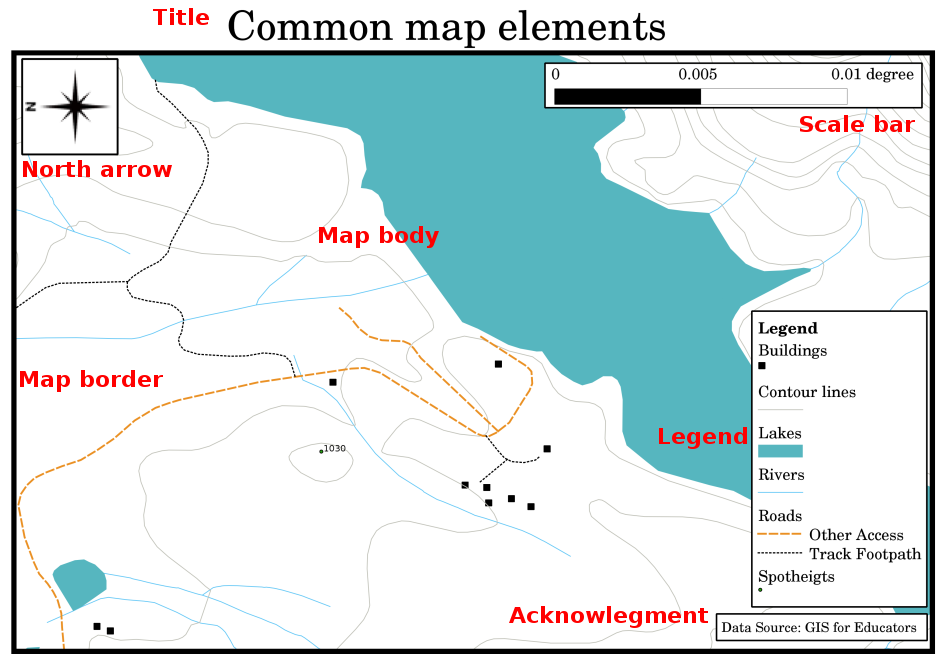
\includegraphics[clip=true, width=0.8\textwidth]{common_map_elements}
\end{center}
\end{figure}

Other elements that might be added are e.g. a \textbf{graticule}, or
\textbf{name of the map projection} (CRS). Together, these elements help the
map reader to interpret
the information shown on the map. The map body is, of course, the most
important part of the map because it contains the map information. The other
elements support the communication process and help the map reader to
orientate himself and understand the map topic. For example, the title
describes the subject matter and the legend relates map symbols to the mapped
data.  

\subsection{Map Title in detail}

The map title is very important because it is usually the first thing a
reader will look at on a map. It can be compared with a title in a newspaper.
It should be short but give the reader a first idea of what the map is about.

\subsection{Map Border in detail}

The map border is a line that defines exactly the edges of the area shown on
the map. When printing a map with a graticule (which we describe further
down), you often find the coordinate information of the graticule lines along
the border lines, as you can see in Figure \ref{fig:maplegends}.
  
\subsection{Map Legend in detail}

A map is a simplified representation of the real world and map
\textbf{symbols} are
used to represent real objects. Without symbols, we wouldn't understand maps.
To ensure that a person can correctly read a map, a map legend is used to
provide a key to all the symbols used on the map. 

\begin{figure}[ht]
   \begin{center}
   \caption{Two maps from the same area, both with a water body in the
background but with different themes, map symbols and colours in the legend.}
\label{fig:maplegends}\smallskip
   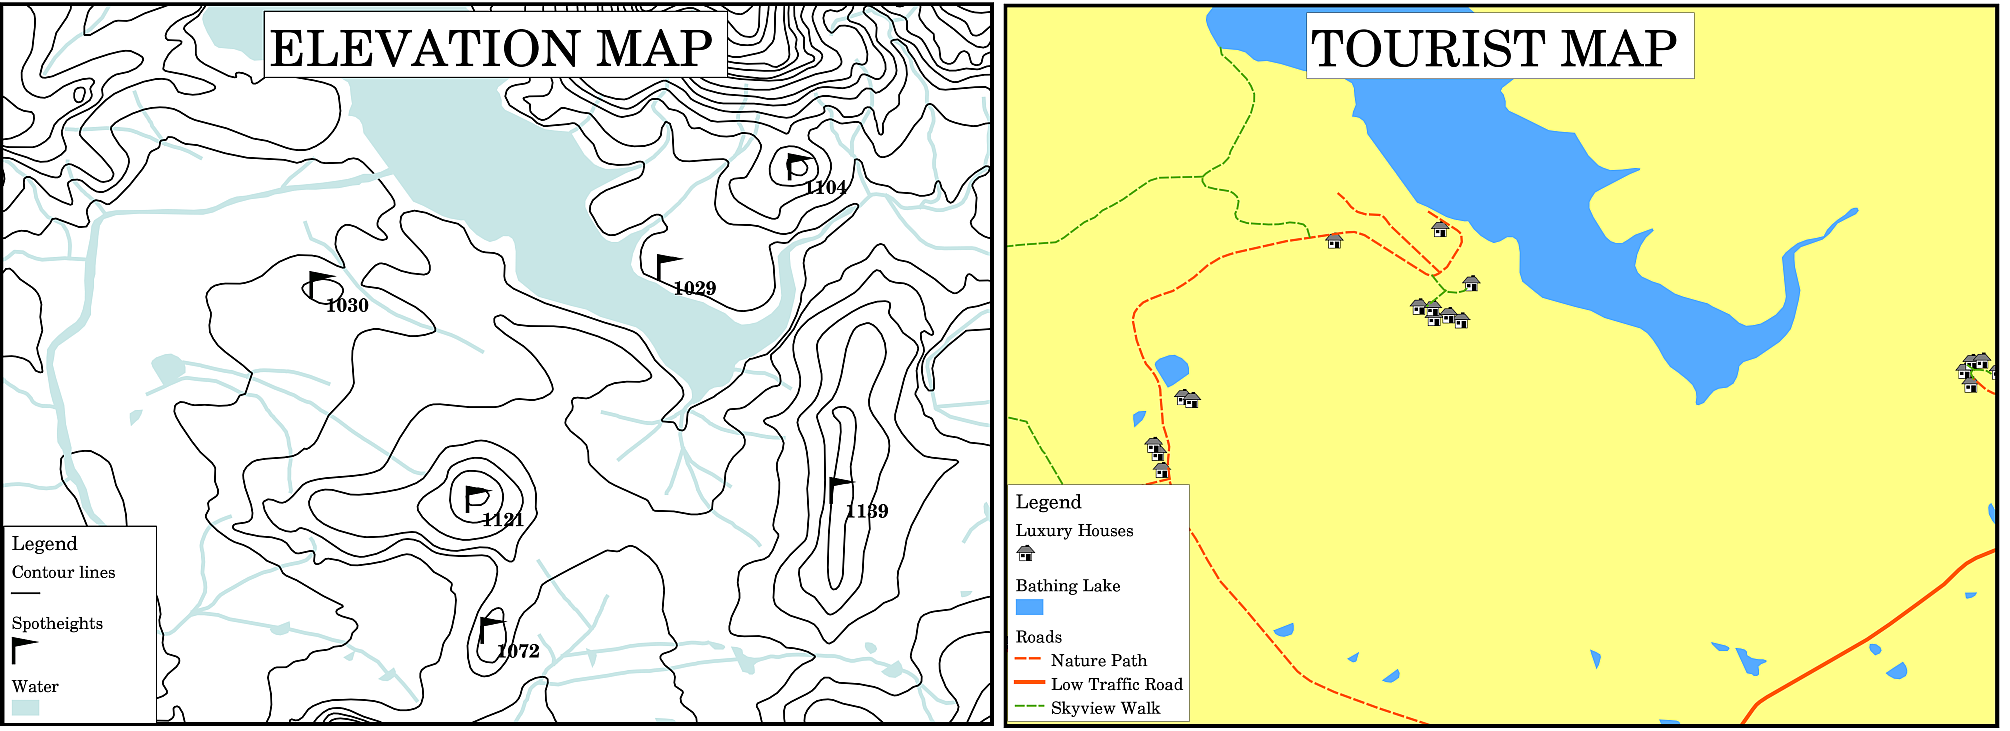
\includegraphics[clip=true, width=0.8\textwidth]{legend-maps}
\end{center}
\end{figure}

It is like a dictionary
that allows you to understand the meaning of what the map shows. A map legend
is usually shown as a little box in a corner of the map. It contains icons,
each of which will represent a type of feature. For example, a house icon
will show you how to identify houses on the map (see Figure
\ref{fig:maplegends}). 

You can also use different symbols and icons in your legend to show different
themes. In Figure \ref{fig:maplegends} you can see a map with a lake in light
blue
overlaid with contour lines and spot heights to show information about the
terrain in that area. On the right side you see the same area with the lake
in the background but this map is designed to show tourists the location of
houses they can rent for their holidays. It uses brighter colours, a house
icon and more descriptive and inviting words in the legend. 

\subsection{North arrow in detail}

A north arrow (sometimes also called a compass rose) is a figure displaying
the main directions, \textbf{North, South, East} and \textbf{West}. On a map
it is used to
indicate the direction of North. 
For example, in GIS this means that a house that is located north from a lake
can be found on top of the lake on a map. The road in the east will then be
to the right of the water body on the map, a river in the south will be below
the water body and if you are searching for a train station to the west of
the lake you will find it on the left side on the map. 

\subsection{Scale in detail}

The scale of a map, is the value of a single unit of distance on the map,
representing distance in the real world. The values are shown in map units
(meters, feet or degrees). The scale can be expressed in several ways, for
example, in words, as a ratio or as a graphical scale bar (see Figure
\ref{fig:scales}).

\textbf{Expressing a scale} in words is a commonly used method and has the
advantage
of being easily understood by most map users. You can see an example of a
word based scale in Figure \ref{}a below. Another option is the
\textbf{representative fraction (RF)} method, where both the map distance and the
ground distance in the real world are given in the same map units, as a
ratio. For example, a RF value 1:25,000 means that any distance on the map is
1/25,000th of the real distance on the ground (see Figure \ref{fig:scales}b below).
The value 25,000 in the ratio is called the \textbf{scale denominator}. More
experienced users often prefer the representative fraction method, because it
reduces confusion. 

When a representative fraction expresses a very small ratio, for example
1:1000 000, it is called a \textbf{small scale map}. On the other hand if the
ratio is
very large, for example a 1:50 000 map, it is called a \textbf{large scale
map}. It is
handy to remember that a small scale map covers a \textbf{large area}, and a
large scale map covers a \textbf{small area}!

A \textbf{scale expression as a graphic or bar scale} is another basic method of
expressing a scale. A bar scale shows measured distances on the map. The
equivalent distance in the real world is placed above as you can see in
Figure \ref{fig:scales}c below. 

\begin{figure}[ht]
   \begin{center}
   \caption{A map scale can be expressed in words (a), as a ratio (b), or as
graphic or bar scale (c).}
\label{fig:scales}\smallskip
   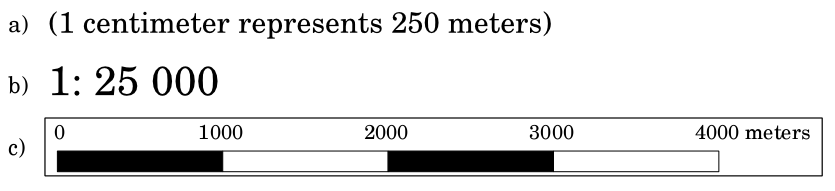
\includegraphics[clip=true, width=0.7\textwidth]{mapscale}
\end{center}
\end{figure}

Maps are usually produced at standard scales of, for example, 1:10 000, 1:25
000, 1:50 000, 1:100 000, 1:250 000, 1:500 000. What does this mean to the
map reader? It means that if you multiply the distance measured on the
\textbf{map} by the \textbf{scale denominator}, you will know the distance in
the \textbf{real world}.

For example, if we want to measure a distance of 100mm on a map with a scale
of 1:25,000 we calculate the real world distance like this:

\begin{table}[ht]
\centering
 \begin{tabular}{|p{6cm}|}
 \hline
 100mm x 25,000 = 2,500,000 mm \\
 \hline
\end{tabular}
\end{table}

This means that 100mm on the map is equivalent to 2,500,000mm (250m) in the
real word. 

\begin{figure}[ht]
   \begin{center}
   \caption{Maps showing an area in two different scales. The map scale on
the left is 1:25,000. The map scale on the right is 1:50,000.}
\label{fig:diffscales}\smallskip
   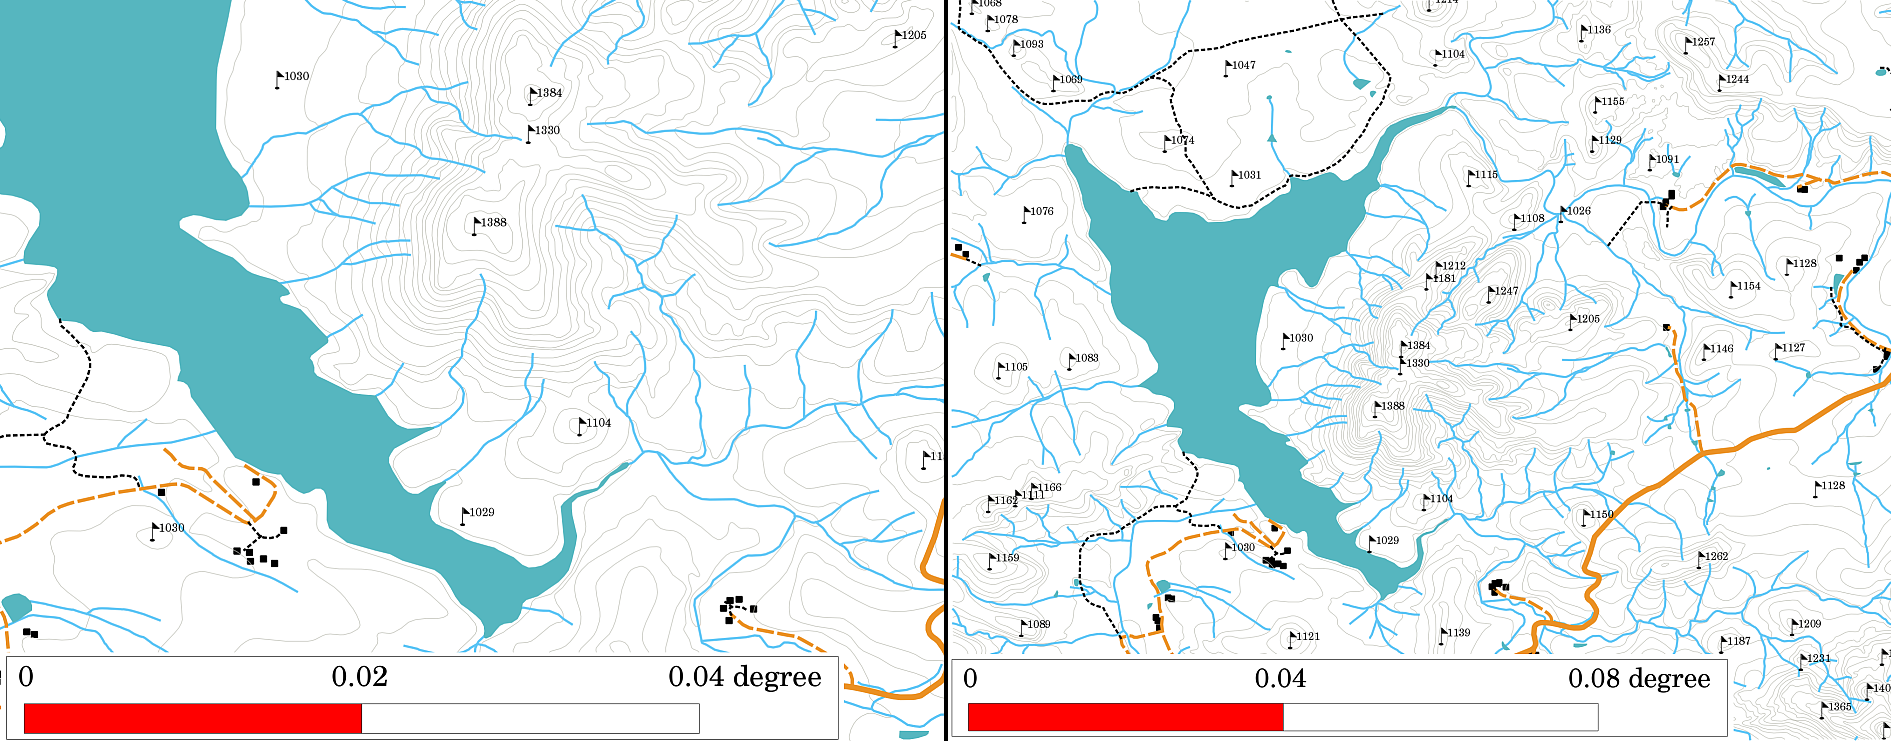
\includegraphics[clip=true, width=\textwidth]{different_scales}
\end{center}
\end{figure}

Another interesting aspect of a map scale, is that the lower the map scale,
the more detailed the feature information in the map will be. In Figure
\ref{fig:diffscales}, you can see an example of this. Both maps are the same
size but have
a different scale. The image on the left side shows more details, for example
the houses south-west of the water body can be clearly identified as separate
squares. In the image on the right you can only see a black clump of
rectangles and you are not able to see each house clearly.

\subsection{Acknowledgment in detail}

In the acknowledgment area of a map it is possible to add text with important
information. For example information about the quality of the used data can
be useful to give the reader an idea about details such as how, by whom and
when a map was created. If you look at a topographical map of your town, it
would be useful to know when the map was created and who did it. If the map
is already 50 years old, you will probably find a lot of houses and roads
that no longer exist or maybe never even existed. If you know that the map
was created by an official institution, you could contact them and ask if
they have a more current version of that map with updated information. 

\subsection{Graticule in detail}

A graticule is a network of lines overlain on a map to make spatial
orientation easier for the reader. The lines can be used as a reference. As
an example, the lines of a graticule can represent the earth's parallels of
latitude and meridians of longitude. When you want to refer to a special area
on a map during your presentation or in a report you could say: 'the houses
close to latitude 26.04 / longitude -32.11 are often exposed to flooding
during January and February' (see Figure \ref{fig:graticule}).

\begin{figure}[ht]
   \begin{center}
   \caption{Graticules (red lines) representing the Earth's parallels of
latitude and meridians of longitude. The latitude and longitude values on the
map border can be used for better orientation on the map.}
\label{fig:graticule}\smallskip
   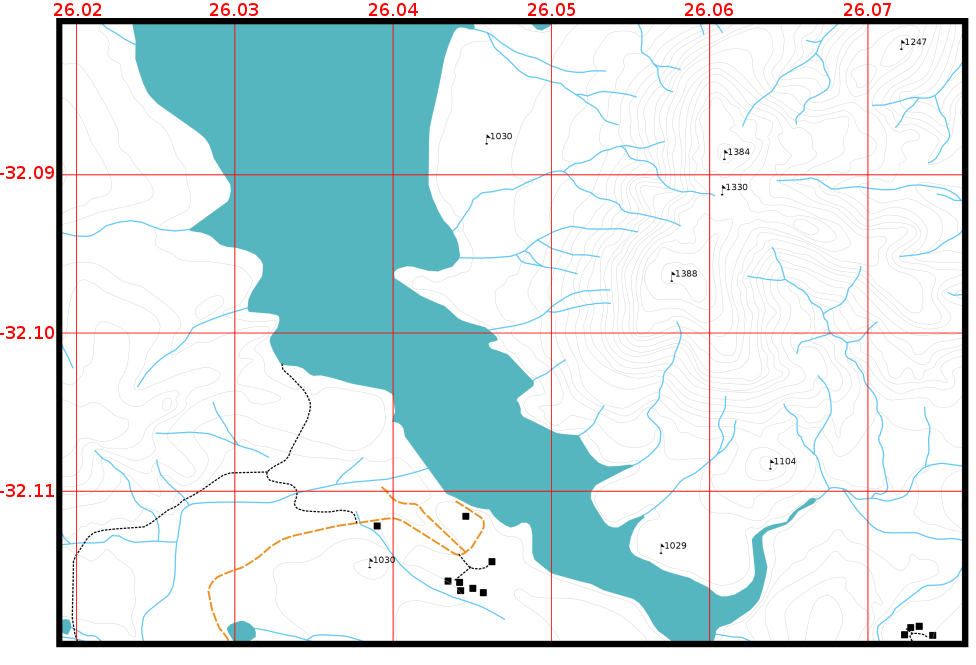
\includegraphics[clip=true, width=0.7\textwidth]{kommandodrif_graticule}
\end{center}
\end{figure}

\subsection{Name of the map projection in detail}

A map projection tries to represent the 3-dimensional Earth with all its
features like houses, roads or lakes on a flat sheet of paper. This is very
difficult as you can imagine, and even after hundreds of years there is no
single projection that is able to represent the Earth perfectly for any area
in the world. Every projection has advantages and disadvantages. 
To be able to create maps as precisely as possible, people have studied,
modified, and produced many different kinds of projections. In the end almost
every country has developed its own map projection with the goal of improving
the map accuracy for their territorial area (see Figure \ref{fig:diffprojs}).

\begin{figure}[ht]
   \begin{center}
   \caption{The world in different projections. A Mollweide Equal Area
projection left, a Plate Carree Equidistant Cylindrical projection on the
right.}
\label{fig:diffprojs}\smallskip
   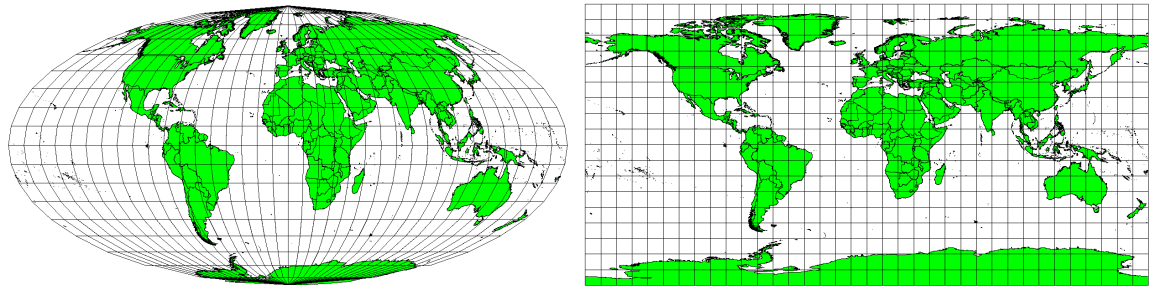
\includegraphics[clip=true, width=\textwidth]{different-projections}
\end{center}
\end{figure}

With this in mind, we can now understand why it makes sense to add the name
of the projection on a map. It allows the reader to see quickly, if one map
can be compared with another. For example, features on a map in a so-called
Equal Area projection appear very different to features projected in a
Cylindrical Equidistant projection (see Figure \ref{fig:diffprojs}). 
    
Map projection is a very complex topic and we cannot cover it completely
here. You may want to take a look at our previous topic: Coordinate Reference
Systems if you want to know more about it.

\subsection{Common problems / things to be aware of}

It is sometimes difficult to create a map that is easy to understand and well
laid out whilst still showing and explaining all the information that the
reader needs to know. To achieve this, you need to create an ideal
arrangement and composition of all the map elements. You should concentrate
on what story you want to tell with your map and how the elements, such as
the legend, scale bar and acknowledgements should be ordered. By doing this,
you will have a well designed and educational map, that people would like to
look at and be able to understand.  

\subsection{What have we learned?}

Let's wrap up what we covered in this worksheet:

\begin{itemize}
\item \textbf{Map production} means arranging map elements on a sheet of paper.
\item \textbf{Map elements} are the title, map body, map border, legend,
scale, north arrow and the acknowledgement.
\item \textbf{Scale} represents the ratio of a distance on the map to the
actual distance in the real world.
\item Scale is displayed in \textbf{map units} (meters, feet or degrees)
\item A \textbf{legend} explains all the symbols on a map.
\item A map should \textbf{explain complex information as simply as possible}. 
\item Maps are usually always displayed \textbf{'North up'}.
\end{itemize}

\subsection{Now you try!}

Here are some ideas for you to try with your learners:

\begin{itemize}
\item Load some vector layers in your GIS for your local area. See if your learners
can identify examples of different types of legend elements such as road
types or buildings. Create a list of legend elements and define what the
icons should look like, so a reader can most easily figure out their meaning
in the map.
\item Create a map layout with your learners on a sheet of paper. Decide on the
title of the map, what GIS layers you want to show and what colours and icons
to have on the map. Use the techniques you learned in Topics 2 and 3 to
adjust the symbology accordingly. When you have a template,  open the QGIS
Map Composer and try to arrange a map layout as planned.
\end{itemize}

\subsection{Something to think about}

If you don't have a computer available, you can use any topographical map and
discuss the map design with your learners. Figure out if they understand what
the map wants to tell. What can be improved? How accurately does the map
represent the history of the area? How would a map from 100 years ago differ
from the same map today?

\subsection{Further reading}

\textbf{Books}: 

\begin{itemize}
\item Chang, Kang-Tsung (2006): Introduction to Geographic Information Systems. 3rd
Edition.  McGraw Hill. (ISBN 0070658986)
\item DeMers, Michael N. (2005): Fundamentals of Geographic Information Systems.
3rd Edition. Wiley. (ISBN 9814126195)
\end{itemize}

\textbf{Websites}:

\url{http://en.wikipedia.org/wiki/Scale\_(map)} \\
\url{http://www.colorado.edu/geography/gcraft/notes/mapproj/mapproj.html}

The QGIS User Guide also has more detailed information on map production
provided in QGIS.

\subsection{What's next?}

In the section that follows we will take a closer look at \textbf{vector
analysis} to see how we can use a GIS for more than just making good looking
maps!

